\section{Згорткові нейронні мережі}

\begin{definition}
    Маскою людини \(F^{i}\) будемо називати бінарне прямокутне
зображення \(M^{i}:P \rightarrow \left\{ 0,1 \right\}\), де тим
пікселям, в яких на відповідному кадрі \(F^{i}\) була помічена людина,
відповідає одиниця, а іншим відповідає нуль.
\end{definition}
Для локалізації людини були використані згорткові нейронні мережі 
(англ. convolutional neural networks, CNN).
В таких мережах застосовується операція згортки (англ. convolution)
та пулінгу (англ. pooling), нормалізація пакетів (англ. batch normalization)
та різні функції активації на кшталт ReLU, Tanh тощо.

Надалі комбінацію (згортка + нормалізація пакетів + функція активації)
будемо називати згортковим шаром, але кожний автор нейронної мережі
створює свої шари, що можуть відрізнятися від вищезазначеного.

\begin{figure}[H]
    \centering
    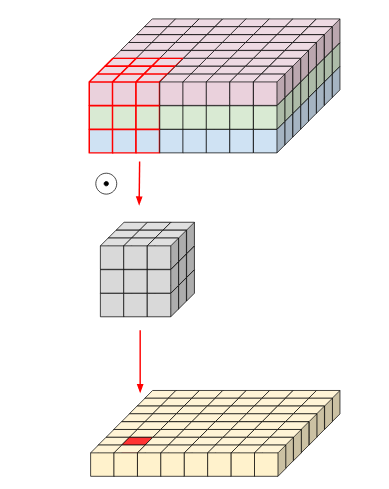
\includegraphics[width=0.3\textwidth]{images/cnn_conv_operation}
    \caption{Ілюстрація взяття згортки  \cite{deep_wise_sep_conv_website}
        \label{fig:cnn:conv_operation}
    }
\end{figure}

Розглянемо архітектури нейронних мереж, які застосовувались у роботі
для локалізації людини. Всі нищеописані нейронні мережі були використані вже з
натренованими вагами у програмній бібліотеці PyTorch \cite{pytorch_library}.
За мету було поставлено підібрати таку мережу, яка здатна швидко та якісно оброблювати
один знімок навіть на смартфоні.

\subsection{YOLO (You Only Look Once)}

YOLO~---~це сімейство нейронних мереж, вперше представлене дослідником на ім'я Joseph Redmon \cite{yolov1}.
Мережа YOLO розв'язує задачу детекції об'єктів як задачу регресії
щодо просторового розділення знайдених областей об'єктів та їх
ймовірностей. Її зараз широко використовують для локалізації та класифікації об'єктів,
оскільки вона здатна оброблювати відео в реальному часі з частотою 30 кадрів в секунду
на мобільних пристроях, що є її найбільшою перевагою серед інших аналогів.

Опишемо коротко принцип роботи YOLOv1, оскільки YOLOv5, яка застосовувалась
в роботі, є її модифікацією.
\begin{enumerate}
    \item Спочатку зображення розділяється решіткою $S \times S$.
          Якщо центр об'єкту потрапляє в комірку решітки, ця комірка
          є кандидатом, для подальшої локалізації об'єкта.
    \item Кожна комірка решітки має передбачувати $B$ областей та рівнів
          довіри. Рівень довіри показує, наскільки модель ``впевнена'',
          що дана комірка містить об'єкт, та наскільки точна область.
          Рівень довіри $t$ визначається  як
          \begin{equation*}
           t = Pr(Object)*{IOU}_{pred}^{truth}, 
          \end{equation*}
          де $Pr(Object)$ ~---~ ймовірність об'єкту, а ${IOU}_{pred}^{truth}$ ~---~ величина
          перетину передбаченої області об'єкту до її справжньої.
          Відповідно, якщо модель не знайшла об'єкт, цей рівень нульовий.
          Необхідно, щоб $t$ був якомога ближчим до ${IOU}_{pred}^{truth}$.
    \item Кожна область об'єкту складається з 5 чисел: рівень довіри,
      $x, y$ (координати центру об'єкту),  $w, h$ (ширина та висота об'єкту).
          Кожна комірка передбачає $C$ умовних ймовірностей $Pr(Class_i|Object)$.
\end{enumerate}

\begin{figure}[H]
    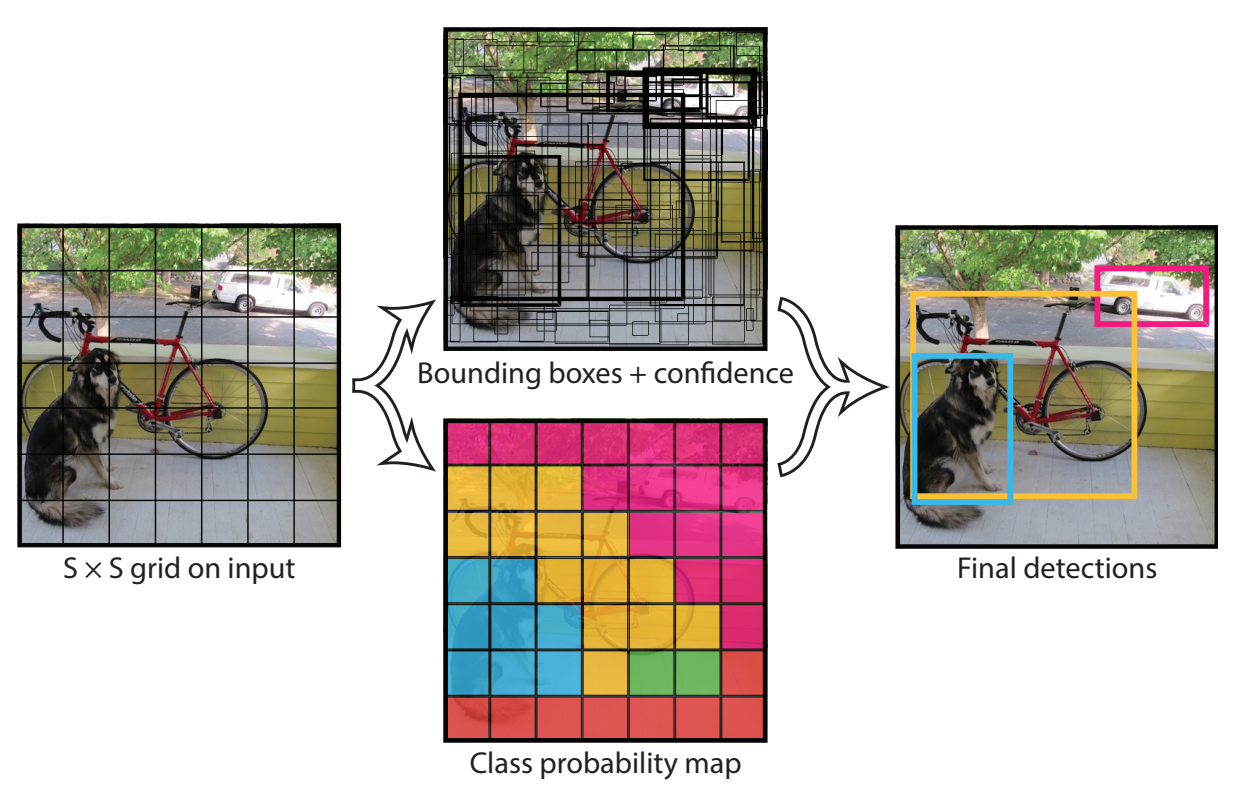
\includegraphics[width=0.5\linewidth]{images/cnn_yolo1}
    \centering
    \caption{Процес локалізації об'єктів мережею YOLOv1 \cite{yolov1}
    }
\end{figure}

Для тренування мережі використовують суму 4 штрафних функцій.

\begin{multline*}
    \lambda_{coord}(
    \underbrace{ \sum_{i=0}^{S^2} \sum_{j=0}^{B}
    \mathds{1}_{ij}^{obj} [(x_i - \widehat{x_i})^2 + (y_i - \widehat{y_i})^2]
    }_\textrm{по координатам центру}\\
    +
    \underbrace{
    \sum_{i=0}^{S^2} \sum_{j=0}^{B}
    \mathds{1}_{ij}^{obj} [(\sqrt{w_i} - \sqrt{\widehat{w_i}})^2 + (\sqrt{h_i} - \sqrt{\widehat{h_i}})^2]
    }_\textrm{ширини та висоти об'єкту}
    )\\
    +  \underbrace{
        \sum_{i=0}^{S^2} \sum_{j=0}^{B} з
        \mathds{1}_{ij}^{obj} (C_i - \widehat{C_i})^2
        +
        \lambda_{noobj} \sum_{i=0}^{S^2} \sum_{j=0}^{B} \mathds{1}_{ij}^{noobj} (C_i - \widehat{C_i})^2
    }_\textrm{точності класифікації}\\
    +  \underbrace{
    \sum_{i=0}^{S^2} \mathds{1}_{i}^{noobj}\sum_{c \in classes}(p_i(c) -  \widehat{p_i}(c))^2
    }_\textrm{ймовірності класів},
\end{multline*}
де $\mathds{1}_{i}^{obj}$ показує, чи знайшовся об'єкт в комірці $i$, а
$\mathds{1}_{ij}^{obj}$ показує, чи в комірці $i$ в $j$-ій області знаходиться об'єкт.

Загалом архітектура нейронної мережі YOLOv1 складається з 24 згорткових шарів та
2 повнозв'язних лінійних шарів.

\begin{figure}[H]
    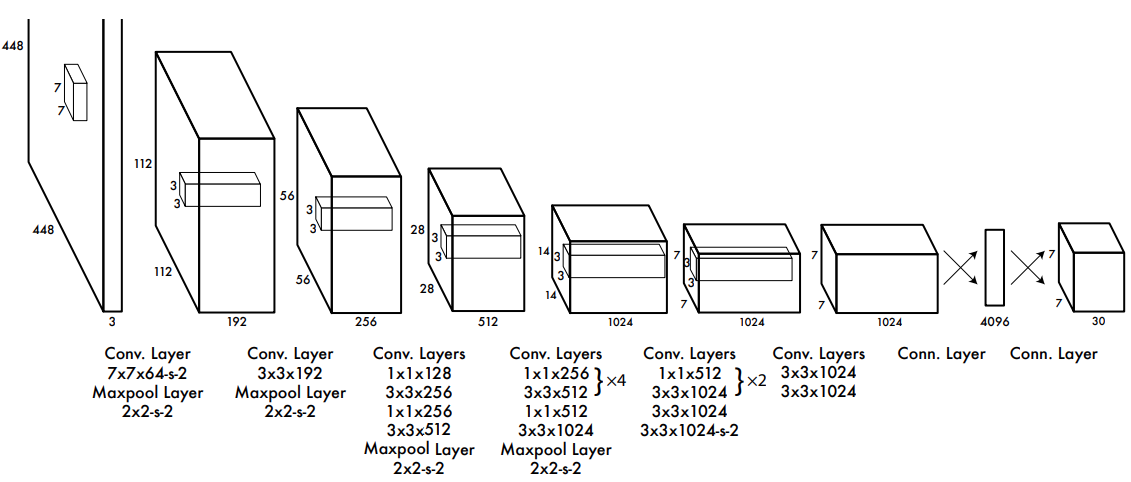
\includegraphics[width=0.8\linewidth]{images/cnn_yolo2}
    \centering
    \caption{Архітектура YOLOv1 \cite{yolov1}
    }
\end{figure}

У поточій роботі була використана одна з мереж YOLOv5, яка була
розроблена Glenn Jocher на програмній бібліотеці PyTorch.

\begin{figure}[H]
    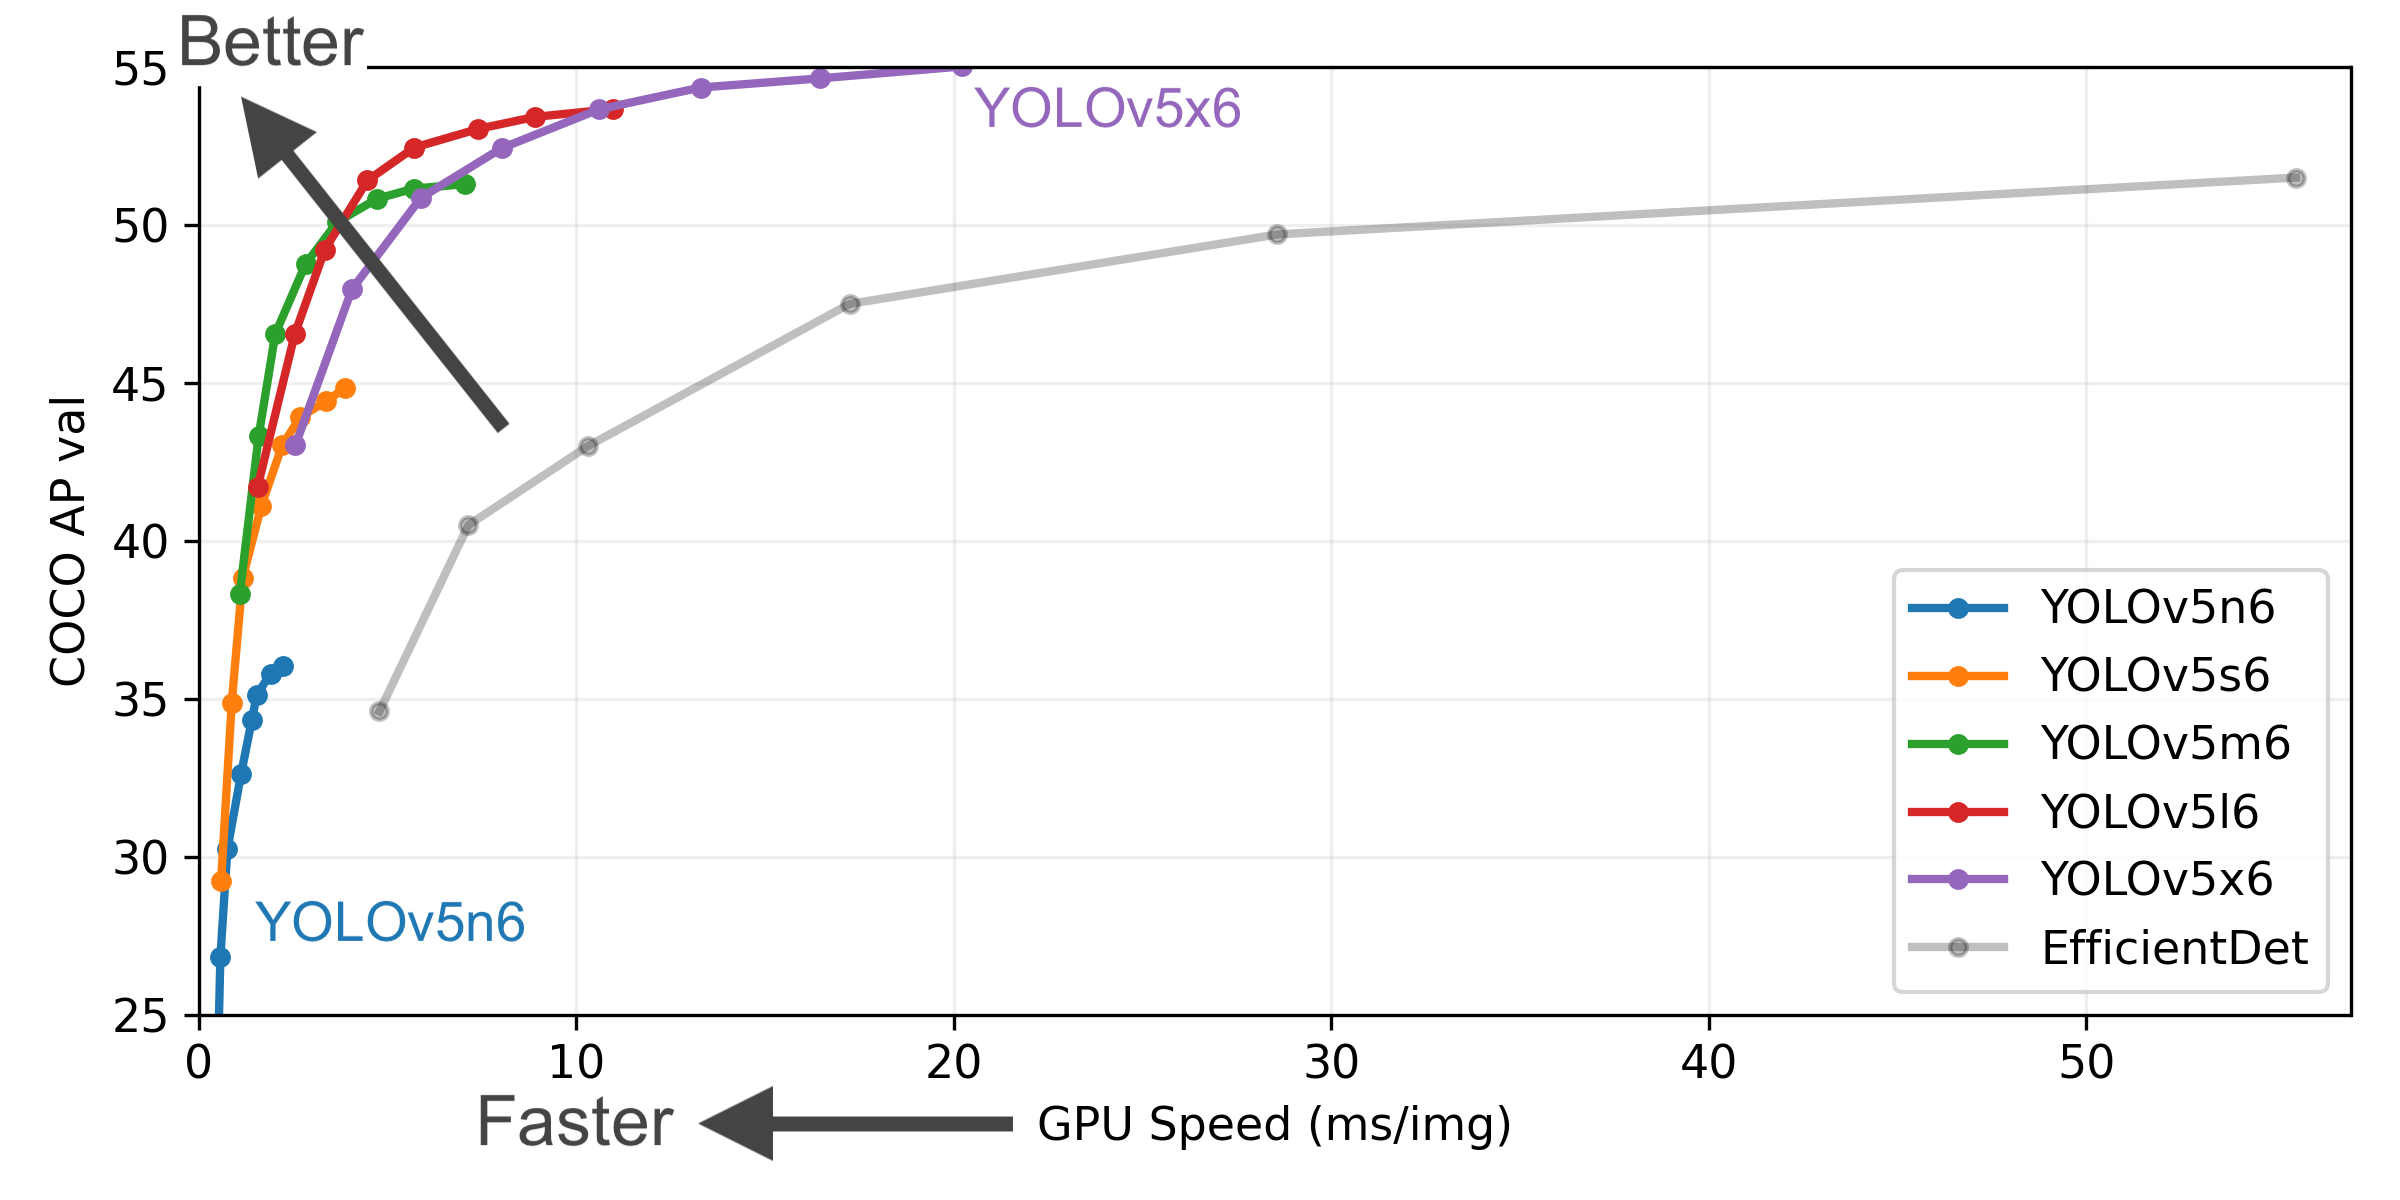
\includegraphics[width=0.5\linewidth]{images/cnn_yolo3}
    \centering
    \caption{Графік залежності точності на датасеті COCO від швидкості обробки однієї
        картинки різними мережами YOLOv5
    }
\end{figure}

\subsection{MobileNet}

MobileNet ~---~ це також ще одне сімейство, що часто використовується у комп'ютерному зорі.
Вперше MobileNetv1 \cite{mobilenetv1} була представлена у 2017 році науковцями з Google.
Мережі даної категорії теж зробили свою революцію в обчисленні глибоких шарів з
використанням мінімальних обчислювальних ресурсів. Були запропоновані два гіперпараметри,
змінивши які можна отримати приріст в швидкості або точності. Мережі MobileNet
застосовуються для локалізації і класифікації об'єктів, а також для широкомасштабної
гео-локалізації.

Розглянемо особливості різних версій MobileNet.

\subsubsection{MobileNetv1}
Однією з головних задач для побудови першої мережі даного сімейства була заміна
звичайного згорткового шару на новий глибинно-просторовий згортковий шар
(англ. depth-wise separable convolution) (рис. \ref{fig:cnn:deep_wise_sep_conv}).

Нехай на вході маємо
\begin{itemize}
    \item квадратне зображення $I$ розмірами $S_I \times S_I \times M$: ширина, висота та
          кількість каналів відповідно;
    \item ядро $C$ розмірами $S_C \times S_C \times M \times N$, де $N$ ~---~ це вихідна розмірність
          отриманої згортки;
    \item вихідна згортка $C$ розмірами $S_K \times S_K \times N$.
\end{itemize}
Тоді формулу звичайної згортки (рис. \ref{fig:cnn:conv_operation}) можна записати як

\begin{equation*}
    G_{k,l,n} = \sum_{i,j,m} C_{i,j,m,n} \cdot  F_{k+i-1, l+j-1,m}.
\end{equation*}
Для обчислення такої згортки потрібно $S_C \cdot  S_C \cdot  M \cdot  N \cdot  S_I \cdot  S_I$ операцій, що
створює обчислювальні обмеження на мобільний пристрій, якщо використовувати
декілька таких згорток.
Для вирішення даної проблеми застосовується глибинна згортка (рис. \ref{fig:cnn:deep_wise_conv}).
Вона полягає у використанні окремої згортки кожного каналу ядра до кожного каналу
зображення.
Нехай $\widehat{C}$~---~ядро глибинної згортки. Тоді
\begin{equation}
    \widehat{G}_{k,l,n} = \sum_{i,j,m} \widehat{C}_{i,j,m,n} \cdot  F_{k+i-1, l+j-1,m}.
\end{equation}
\begin{figure}[H]
    \centering
    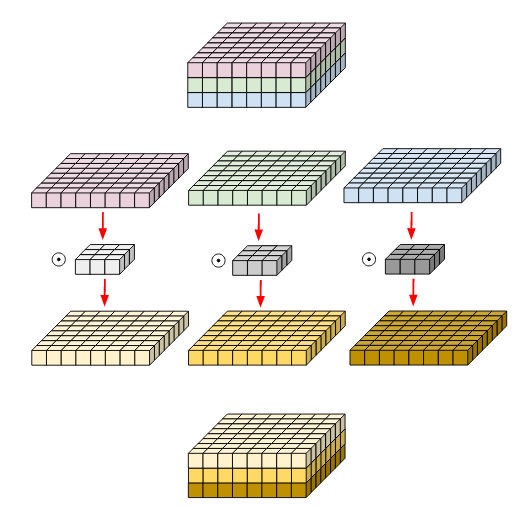
\includegraphics[width=0.35\textwidth]{images/cnn_deep_wise_conv}
    \caption{Ілюстрація взяття глибинної згортки  \cite{deep_wise_sep_conv_website}
        \label{fig:cnn:deep_wise_conv}
    }
\end{figure}
Для обчислення такої згортки потрібно  $S_C \cdot  S_C \cdot  M \cdot  S_I \cdot  S_I$ операцій. Ми вже 
позбулись $N$ операцій, але маємо пам'ятати, що
зараз $\widehat{G}$ складається з $M$ окремих вихідних згорток.
тому, щоб створити єдиний вихід, додатково до глибинної застосовують ще
й точкову згортку (англ. point-wise convolution), в якій розмір
ядра $1 \times 1$. Тоді маємо
$S_C \cdot  S_C \cdot  M \cdot  S_I \cdot  S_I + M \cdot  N \cdot  S_I \cdot  S_I$ операцій.
Дана комбінація має назву глибинно-просторова згортка, для
обчислення якої потрібно в $1/N + 1/S_C^2$ менше операцій, ніж
для звичайної.
\begin{figure}[H]
    \centering
    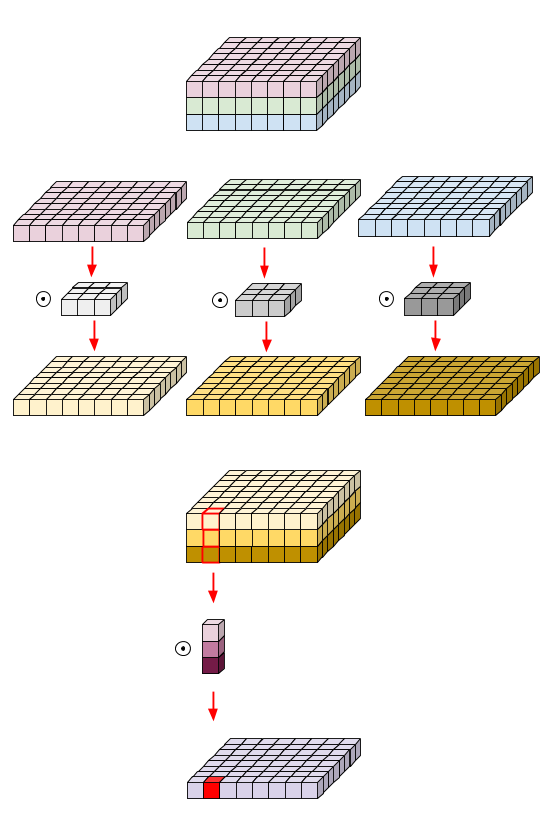
\includegraphics[width=0.35\textwidth]{images/cnn_deep_wise_separable_conv}
    \caption{Ілюстрація взяття глибинно-просторової згортки  \cite{deep_wise_sep_conv_website}
        \label{fig:cnn:deep_wise_sep_conv}
    }
\end{figure}

Таке нововведення в галузі глибокого навчання дало змогу в рази пришвидшити
навчання та роботу не лише згорткової мережі MobileNetv1, а й інших. У MobileNetv1 застосовуються
просторово глибинні згортки з розміром ядра $3 \times 3$.
Маємо таку заміну блоку, як показано на рис. \ref{fig:cnn:mobilenetv1_conv_layer}.

\begin{figure}[H]
    \centering
    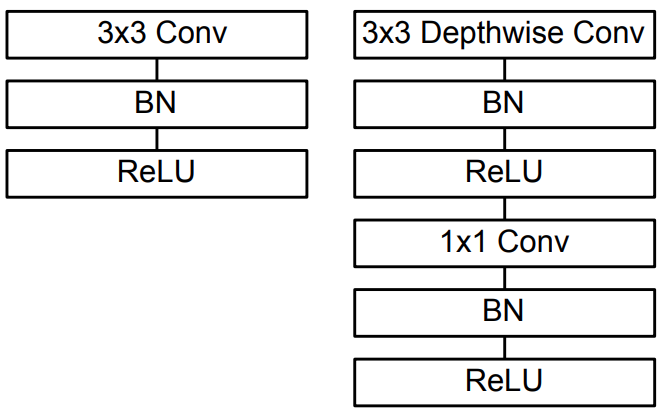
\includegraphics[width=0.4\textwidth]{images/cnn_mobilenetv1_conv_layer}
    \caption{Ліворуч звичайний згортковий шар,
        праворуч згортковий шар у MobileNetv1  \cite{mobilenetv1}
        \label{fig:cnn:mobilenetv1_conv_layer}
    }
\end{figure}

MobileNetv1 має також два гіперпараметра ширини та розмірності.
Множник ширини $\alpha$ застосовується, щоб зменшити кожен шар мережі, що
в свою чергу дає приріст у швидкості.
Iз множником  $\alpha \in (0,1]$ потрібно буде зробити
$S_C \cdot  S_C \cdot  \alpha M \cdot  S_I \cdot  S_I + \alpha M \cdot  \alpha N \cdot  S_I \cdot  S_I$ операцій.
Множник розмірності $\rho$ зменшує вхідну картинку і відповідно
розмірність згорток. Разом із $\alpha$ та $\rho \in (0,1]$ необхідно буде
$S_C \cdot  S_C \cdot  \alpha M \cdot  \rho S_I \cdot  \rho S_I + \alpha M \cdot \alpha  N \cdot  \rho S_I \cdot  \rho S_I$
операцій.

На рис \ref{fig:cnn:mobilenetv1_architecture} можна побачити повну архітектуру мережі MobileNetv1.

\begin{figure}[H]
    \centering
    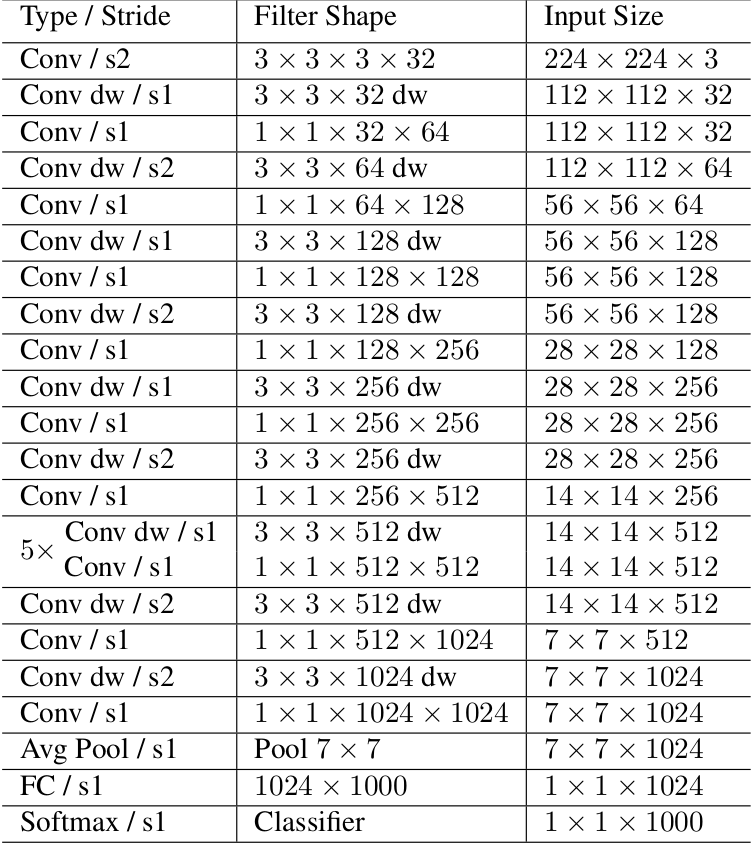
\includegraphics[width=0.4\textwidth]{images/cnn_mobilenetv1_architecture}
    \caption{Архітектура нейронної мережі MobileNetv1   \cite{mobilenetv1}
        \label{fig:cnn:mobilenetv1_architecture}
    }
\end{figure}

\subsubsection{Mobilenetv2}

Вже у 2018 році з'являється 2-га версія мережі MobileNet. У ній автори додали нові зміни в
архітектуру, такі як інвертовані залишки (англ. inverted residuals) та 
лінійні вузькі місця (англ. linear bottlenecks).

Автори зробили дослідження щодо застосування функції ReLU (rectified linear unit) в
контексті низьких розмірностей. Вводиться поняття різноманітності інтересів  (англ. manifold of interest), 
яке автори пояснюють як множину шарів активацій. Була висунута гіпотеза про те що,
різноманітність інтересів з високою розмірністю можна стиснути у підпростір меншої розмірності
зі збереженням інформації.

Розпишемо детальніше кроки, з яких складається новий структурний шар.   
\begin{enumerate}
    \item Нехай на вхід першого розширюючого блоку подається зображення розмірами $S_I \times S_I \times M$.
          Головна особливість цього блоку ~---~ це новий параметр $t$, що називається розширюючим фактором.
          Найкращими значеннями для нього є $[5,10]$. Менші значення краще застосовувати для меншої мережі,
          а більші відповідно для більших. Саме тут використовується різноманітність інтересів.
          Вихід блоку розміром $S_I \cdot  S_I \cdot  (t\cdot M)$.
      \item Наступним кроком є глибинна згортка з функцією активації,
          яка обчислюється за формулою $ReLU6(x) =  min(max(0,x),6)$.
          Вхід розміром $S_I \cdot  S_I \cdot  (t\cdot M)$, а вихід $(S_I/stride) \cdot  (S_I/stride) \cdot  (t\cdot M)$, 
          де  $stride$ ~---~ крок згортки.
    \item Далі застосовується точкова згортка, щоб створити єдиний тензор. На 
          рис. \ref{fig:cnn:mobilenetv2_layer} наведено використання residual block, де вхід у шар
          поєднується з передостаннім блоком.
\end{enumerate}
\begin{figure}[H]
    \centering
    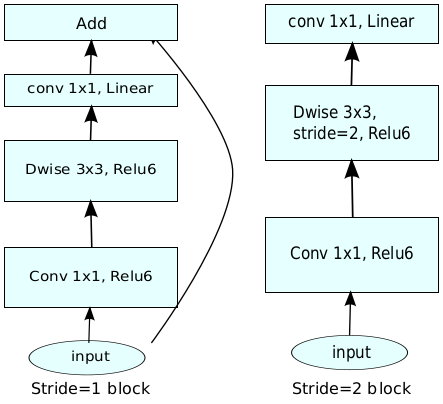
\includegraphics[width=0.5\textwidth]{images/cnn_mobilenetv2_layer}
    \caption{Відмінність MobileNetv2 від MobileNetv1: ліворуч структурний блок MobileNetv2,
        праворуч - MobileNetv1   \cite{mobilenetv2}
        \label{fig:cnn:mobilenetv2_layer}
    }
\end{figure}

\begin{figure}[H]
    \centering
    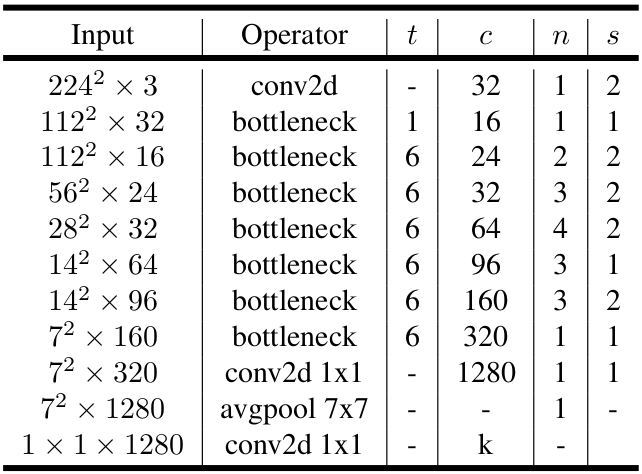
\includegraphics[width=0.5\textwidth]{images/cnn_mobilenetv2_architecture}
    \caption{Архітектура мережі MobileNetv2     \cite{mobilenetv2}
        \label{fig:cnn:mobilenetv2_architecture}
    }
\end{figure}

Варто відмітити, що автори вдосконалили мережу SSD \cite{ssd} шляхом заміни 
звичайних згорткових шарів на розширюючі, які 
використовуються у MobileNetv2. Таким чином створили нову мережу SSDLite \cite{mobilenetv2}.

\subsubsection{MobileNetv3}

На сьогодні останньою є третя версія архітектури сімейства нейронні мереж MobileNet \cite{mobilenetv3}.
Тут автори представили вже дві нейронні мережі MobileNetv3-Small та MobileNetv3-Large.
Це зроблено для того, щоб використовувати модель на слабких і потужних пристроях.
Як запевняють автори, MobileNetV3-Small на 6.6 \% точніша за MobileNetv2, а локалізація об'єктів
з MobileNetV3-Large на COCO датасеті на 25 \% швидша з тією  ж точністю.
Головний блок мережі знову змінився. Розробники взяли
до уваги певні особливості мережі MnasNet, в якій є блок стиснення та збудження
(англ. squeeze and excitation). Мережі з такими блоками називаються Se-Nets.

Мета підходу стиснення та збудження (рис. \ref{fig:cnn:senet_block}) полягає в тому, щоб взяти параметри 
виходу згортки ($u_c$ розмірами $C \times H \times W$)
як вхід блоку стиснення та збудження,
потім зробити операцію стиснення (маємо $1 \times 1 \times C$), операцію збудження ($1 \times 1 \times C$) та 
в кінці масштабувати параметри.
Ідея полягає в тому, щоб підвищити чутливість мережі до інформативних ознак,
і передавати отриману інформацію наступному шару.

\begin{figure}[H]
    \centering
    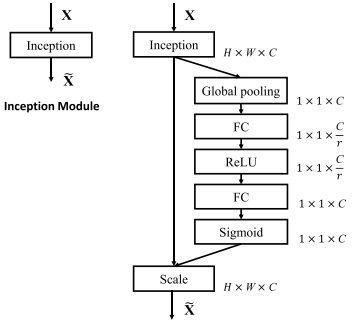
\includegraphics[width=0.5\textwidth]{images/cnn_senet_block}
    \caption{Блок стиснення та збудження      \cite{squeeze_and_excitation_website}
        \label{fig:cnn:senet_block}
    }
\end{figure}

Опишемо блок стиснення та збудження.
\begin{enumerate}
    \item Операція стиснення полягає у відокремленні глобальної інформації з кожного каналу
          вхідного зображення. Дана операція є краща за звичну згортку, оскільки забирає всю інформацію
          з каналу зображення за один раз. Також, операція стиснення відома під назвою глобального
          середнього пулінгу  (англ. global average pooling), яка означає взяття середнього значення 
          по кожному каналу.
          \begin{equation*}
              z = F_{sq}(u_c) = \frac{\sum_{i=0}^{H} \sum_{j=0}^{W} u_c(i,j)}{H\cdot W}.
          \end{equation*}
          Вихід розміром $1 \times 1 \times C$.
    \item Операція збудження створює множину ваг для кожного каналу шляхом застосування
          активацій $Sigmoid$ та $ReLU$ для двох повнозв'язних лінійних шарів.
          \begin{equation*}
              s = F_ex(z,W) = Sigmoid(FC_2ReLu(FC_1z))
          \end{equation*}
          Перший лінійний шар $FC_1$ використовується для зменшення розмірності $z$ з деяким
          множником $r$, тому після нього розмір тензора $1 \times 1 \times C/r$, а $FC_2$ навпаки
          для збільшення $ReLU(W_1 \cdot  z)$. Знаючи, що значення сигмоїди від 0 до 1, можна
          масштабувати її вихід та поєднати із входом в блок стиснення і збудження.
          \begin{equation*}
              \widetilde{x_c} = F_{scale}(u_c,s_c) = s_c\cdot u_c
          \end{equation*}
\end{enumerate}

Автори покращили даний підхід у своїй MobileNetv3, але з використанням
різної нелінійності на кожному шарі. Тут мається на увазі заміна лінійних функцій активацій.
Було вирішено замість нелінійної функції
\begin{equation*}
    swish(x) = x\cdot Sigmoid(x)
\end{equation*}
використати
\begin{equation*}
    h-swish(x) = x\cdot \frac{ReLU6(x + 3)}{6}.
\end{equation*}
Це пов'язано з тим, що сигмоїда для великих тензорів складна в обчисленні 
для малопотужних пристроїв. Автори помітили, 
що використання $h-swish(x)$ дає приріст в точності, якщо її
використовувати у глибоких шарах мережі.

Так само як і у MnasNet \cite{mnasnet}, автори MobileNetv3 використали платформу NAS (neural
architecture structure), яка створена для підбирання глобальних параметрів мережі.
Тобто NAS рекомендує найкращу знайдену архітектуру, а далі NetAdapt \cite{netadapt} (схожа до NAS) допомагає у підборі
параметрів вже всередині одного обчислювального блоку.

Всі вищеописані техніки допомогли створити MobileNetv3-Small та MobileNetv3-Large
(рис. \ref{fig:cnn:mobilenetv3_architecture}).

\begin{figure}[H]
    \centering
    \begin{subfigure}[c]{0.4\textwidth}
        \centering
        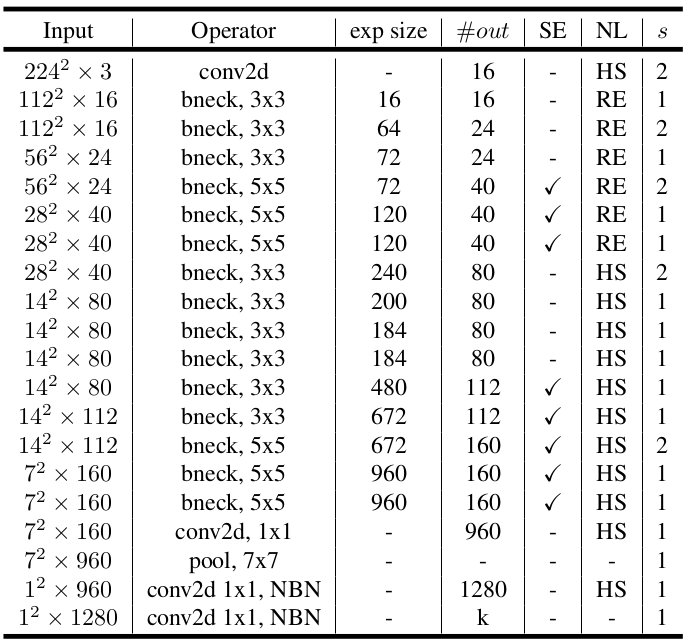
\includegraphics[width=\textwidth]{images/cnn_mobilenetv3_large_architecture}
        \caption{MobileNetv3-Large
        }
    \end{subfigure}
    \begin{subfigure}[c]{0.4\textwidth}
        \centering
        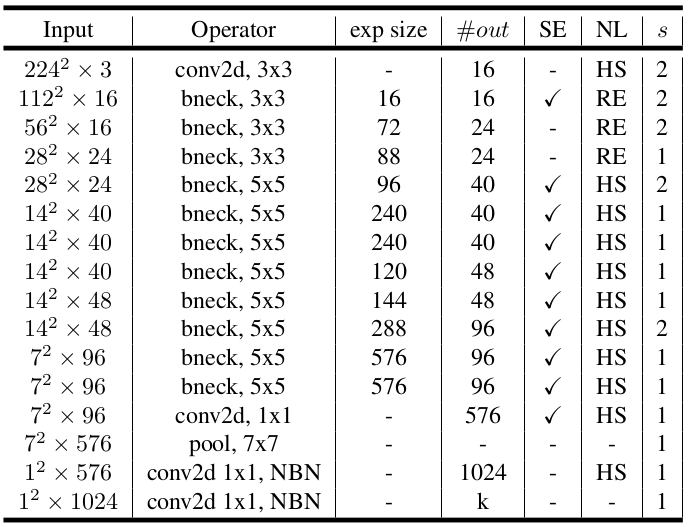
\includegraphics[width=\textwidth]{images/cnn_mobilenetv3_small_architecture}
        \caption{MobileNetv3-Small
        }
    \end{subfigure}
    \caption{Дві архітектури мережі MobileNetv3 \cite{mobilenetv3}
        \label{fig:cnn:mobilenetv3_architecture}
    }
\end{figure}

\subsubsection{SSD (Single Shot Multibox Detector)}

Оскільки для відокремлення ознак в цій роботі застосовується SSD зі
структурними елементами MobileNetv3, покажемо, як саме SSD вдається
локалізувати об'єкти, та його відмінності від YOLO.
Мережа SSD (рис. \ref{fig:cnn:ssd_architecture}), на відміну від YOLO, пропускає зображення
через шари лише один раз. Це пояснюється словами в назві single shot. 
SSD використовує задачу MultiBox регресії локалізованих областей, тому розпишемо її детальніше.
\begin{figure}[H]
    \centering
    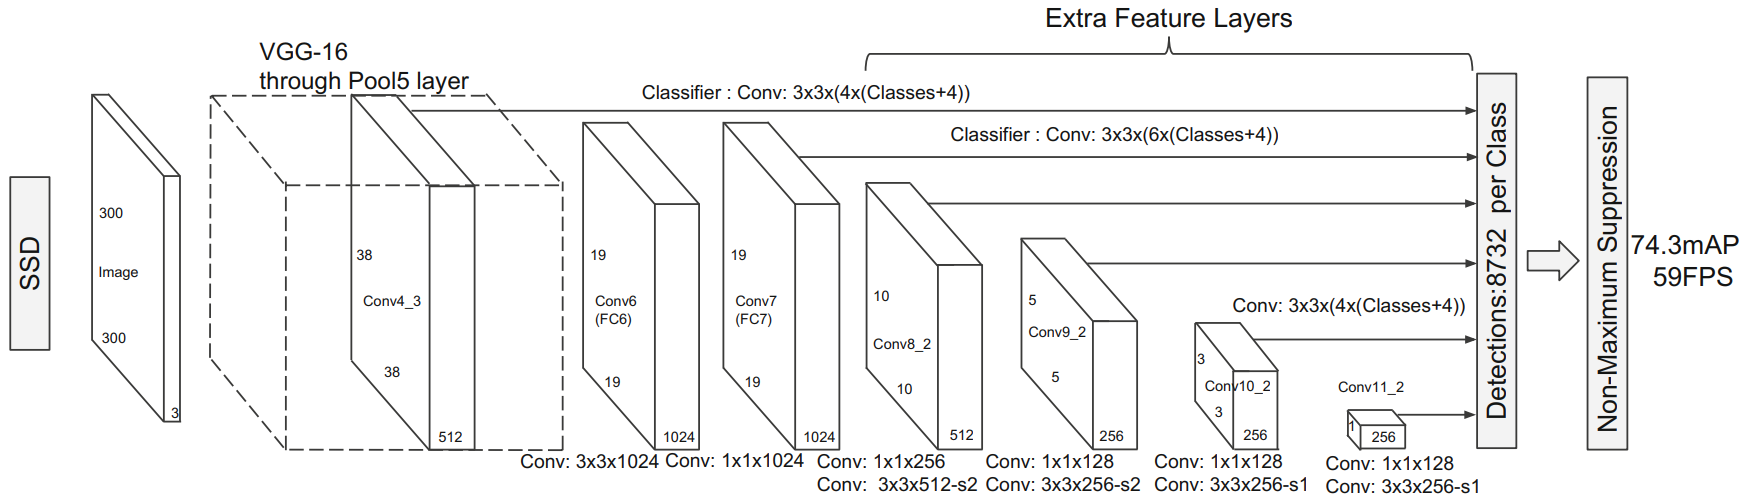
\includegraphics[width=0.8\textwidth]{images/cnn_ssd_architecture}
    \caption{Архітектура мережі SSD на основі VGG-16    \cite{ssd}
        \label{fig:cnn:ssd_architecture}
    }
\end{figure}
Головна задача MultiBox ~---~ оцінити, як локалізувати об'єкти точно. Для цього використовуються
дві штрафні функції. Функція довіри, в основі якої лежить категоріальна перехресна ентропія, та
функція локалізації з $L_2$ нормою, яка показує, наскільки добре справжня область об'єкту співпадає
зі спрогнозованою.
SSD застосовує фіксовані області для подальшого передбачення
зі згортками малого ядра.
Чим більше фіксованих областей, тим більша точність локалізації об'єкту,
але тим довша обробка фото.

Принцип відокремлення інформативних ознак SSD полягає у розбитті зображення на решітку
(рис. \ref{fig:cnn:ssd_work_example}) (аналогічно YOLO). Запускається класифікатор
і вирішує, чи брати ту чи іншу клітинку у якості кандидата на локалізацію. 
Для кожної фіксованої області обчислюється розмір
області та рівень довіри для кожної категорії об'єктів.

\begin{figure}[H]
    \centering
    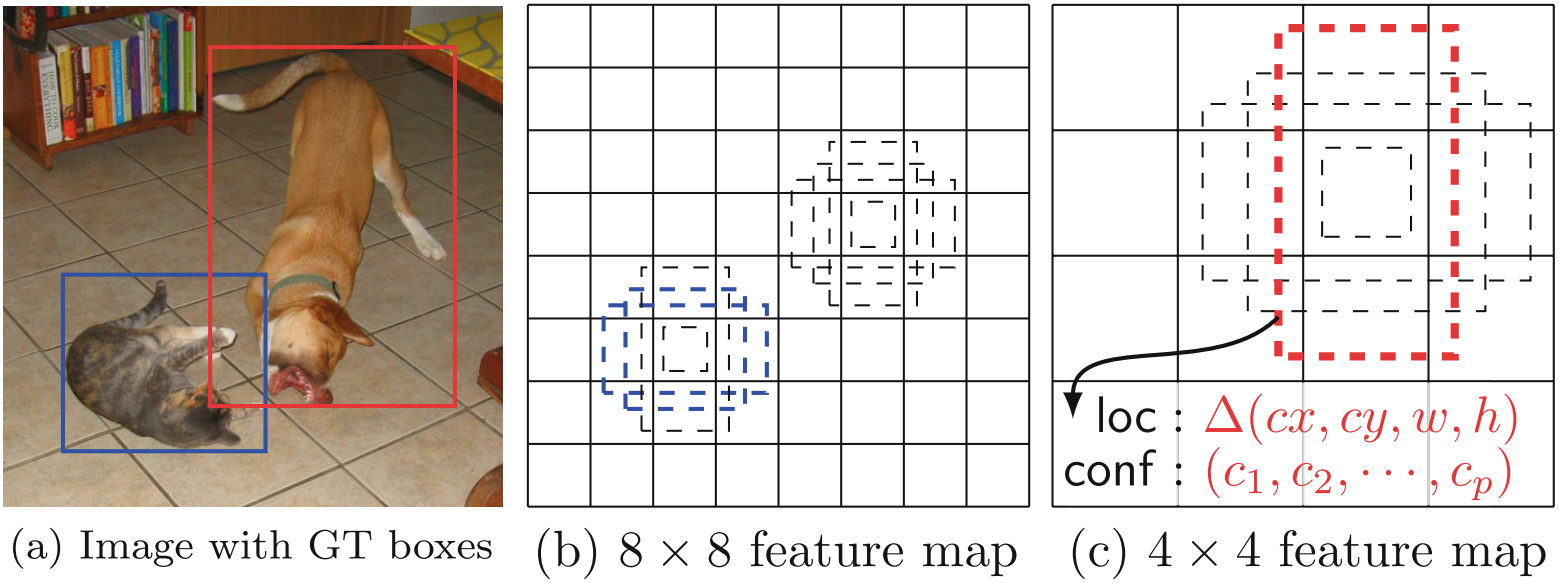
\includegraphics[width=0.7\textwidth]{images/cnn_ssd_work_example}
    \caption{Приклад роботи SSD для локалізації об'єктів \cite{ssd}
        \label{fig:cnn:ssd_work_example}
    }
\end{figure}


\subsubsection{Faster R-CNN}

Говорячи про детекцію і класифікацію об'єктів, не можна обійти увагою інший відомий
клас згорткових нейронних мереж, що має назву R-CNN (region-based convolutional neural network).

Перша мережа R-CNN складалась з 3 незалежних етапів.
На першому генерується 2000 пропозицій областей за допомогою
вибіркового пошуку. Далі ці області проходять стиснення розміру до наперед заданого.
Останній етап ~---~ це метод опорних векторів з заздалегідь натренованими
вагами, який і проводить класифікацію.

R-CNN не була досить потужною, оскільки використовувала вибірковий пошук,
який займає чимало часу. Також потрібно зберігати чимало
кешованих даних для натренованої мережі.

Багато проблем було вирішено вже з новою Fast R-CNN. Вся архітектура складається з одного модуля, 
що в рази полегшує навчання. Тут з'являється новий шар ROI Pooling, головна ціль якого ~---~
надати вектори ознак фіксованої довжини. Даний шар розбиває кожний запропонований
регіон на решітку, в кожній клітинці потім ми знаходимо максимальне значення
(операція max pooling). Але в Fast R-CNN досі
лишився вибірковий алгоритм.

У Faster R-CNN \cite{faster_rcnn} (який теж тестувався для локалізації людини в
цій роботі) автори використали RPN (Region Proposal Network) як спосіб
генерації областей-кандидатів та Fast R-CNN для виявлення об'єктів в цих областях.
Ці два етапи поєднуються в одну мережу за допомогою сумісного використання ознак (feature sharing).
RPN приймає на вхід картинку і повертає множину координат прямокутних областей
(кандидатів для класифікації) з мірами в них присутності об'єкту. RPN ~---~ повнозв'язна
згорткова мережа, що означає, що в ній немає лінійних шарів. Саме вона стала заміною
вибіркового алгоритму у Fast R-CNN.

\begin{figure}[H]
    \centering
    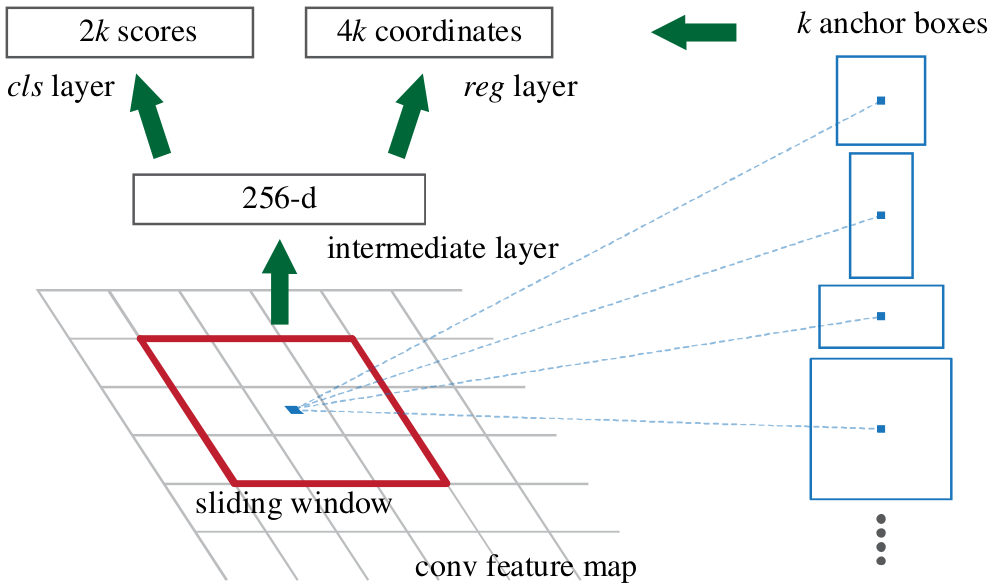
\includegraphics[width=0.5\textwidth]{images/cnn_faster_rcnn_rpn}
    \caption{Архітектура мережі RPN \cite{faster_rcnn}
        \label{fig:cnn:faster_rcnn_rpn}
    }
\end{figure}
RPN використовує принцип ковзкого вікна (sliding window) на згортковій мапі ознак,
отриманої після останнього згорткового шару. Кожне таке вікно відображається
на вектор меншої розмірності. Для кожного вікна генеруються прямокутні області-кандидати,
що називаються опорними регіонами (anchor boxes) з параметрами масштабу та співвідношення сторін.
Далі цей вектор подається на вхід двом повнозв'язним
шарам локалізації об'єктів (box-regression layer) та класифікації (box-classification layer).
Використання опорних регіонів дозволяє детектувати об'єкти практично будь-якого масштабу та
пов'язувати ознаки RPN з Fast R-CNN.

Як вже було сказано, за допомогою принципу поширення ознак можна використовувати вихід RPN як вхід в Fast R-CNN.
Головна його ідея полягає у використанні одних і тих же згорток у двох мережах, що дозволяє тренувати
RPN разом з Fast R-CNN, а не окремо.

\begin{figure}[H]
    \centering
    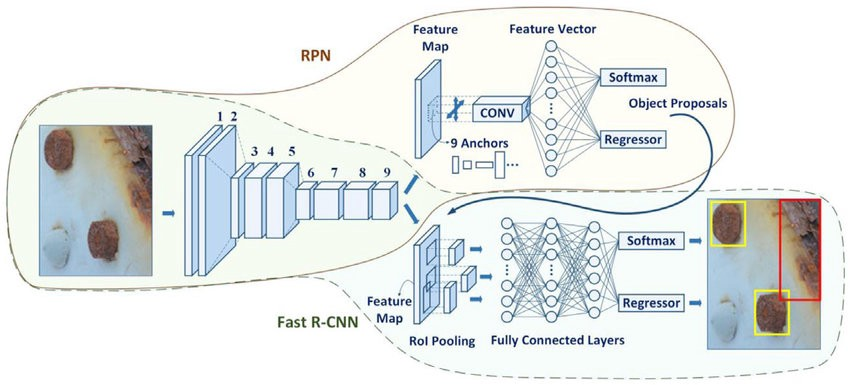
\includegraphics[width=0.7\textwidth]{images/cnn_faster_rcnn_architecture}
    \caption{Архітектура мережі Faster R-CNN \cite{faster_rcnn_web_article}
        \label{fig:cnn:faster_rcnn_architecture}
    }
\end{figure}
\clearpage
